\documentclass{article}

\usepackage{amsthm}
\usepackage{amsfonts}

\usepackage{amsmath}
\usepackage{amssymb}
\usepackage{fullpage}
\usepackage[utf8]{inputenc}
\usepackage{graphicx}
\usepackage[linguistics]{forest}
\usepackage[usenames]{color}
\usepackage{hyperref}
  \hypersetup{
    colorlinks = true,
    urlcolor = blue,       % color of external links using \href
    linkcolor= blue,       % color of internal links 
    citecolor= blue,       % color of links to bibliography
    filecolor= blue,        % color of file links
    }
    
\usepackage{listings}

\definecolor{dkgreen}{rgb}{0,0.6,0}
\definecolor{gray}{rgb}{0.5,0.5,0.5}
\definecolor{mauve}{rgb}{0.58,0,0.82}

\lstset{frame=tb,
  language=haskell,
  aboveskip=3mm,
  belowskip=3mm,
  showstringspaces=false,
  columns=flexible,
  basicstyle={\small\ttfamily},
  numbers=none,
  numberstyle=\tiny\color{gray},
  keywordstyle=\color{blue},
  commentstyle=\color{dkgreen},
  stringstyle=\color{mauve},
  breaklines=true,
  breakatwhitespace=true,
  tabsize=3
}

\theoremstyle{theorem} 
   \newtheorem{theorem}{Theorem}[section]
   \newtheorem{corollary}[theorem]{Corollary}
   \newtheorem{lemma}[theorem]{Lemma}
   \newtheorem{proposition}[theorem]{Proposition}
\theoremstyle{definition}
   \newtheorem{definition}[theorem]{Definition}
   \newtheorem{example}[theorem]{Example}
\theoremstyle{remark}    
  \newtheorem{remark}[theorem]{Remark}


\title{CPSC-354 Report}
\author{Darren Pak  \\ Chapman University}

\date{\today}

\begin{document}

\maketitle

\begin{abstract}
This is a culmination of all assignments and reports for CPSC-354 taught by Alex Kurz at Chapman University Fall 2022. 
\end{abstract}

\tableofcontents

\section{Introduction}\label{intro}

My name is Darren Pak and I am a computer science major at Chapman University with a minor in Data Analytics. My current goals as of Fall 2022 are to find interesting job opportunities and career paths that I find enjoyable and are able to sustain my lifestyle. 

\section{Homework}\label{homework}

This section contains solutions to homework assignments. 

\subsection{Week 1}

In Week 1, I will go over Euclid's Algorithm for Greatest Common Divisor and how it is implemented in C++.

\subsubsection{Euclid's Algorithm}

Euclid's Algorithm is defined as follows:

\medskip\noindent 
gcd(a,b):

\medskip\noindent 
Input: Two whole numbers (integers) called a and b, both greater than 0.

\medskip\noindent 
(1) if $$a > b$$ then replace a by a-b and go to (1).

\medskip\noindent 
(2) if $$b > a$$ then replace b by b-a and go to (1).

\medskip\noindent 
Output: a

\medskip\noindent
As described in \href{https://hackmd.io/@alexhkurz/SkqMtH0sK}{Alex Kurz Homework (Week 1)}

\subsubsection{Implementation in C++}

Below is the example for implementation of Euclid's Algorithm in C++:
\begin{lstlisting}
#include <iostream>

using namespace std;

int gcd(int a, int b) {
    while ((a != 1) && (b != 1)) {
        if (a > b) {
            a = a-b;
        }
        if (b > a) {
            b = b-a;
        }
        if (a == b) {
            return a;
        }
    }
    return a;
}

int main()
{
    cout<<gcd(9,33)<<endl;

    return 0;
}
\end{lstlisting}
In the function gcd, there is a while loop checking if either of the inputs are 1. This will eliminate cases where the GCD is already the lowest possible and as described in Euclid's algorithm, will return 1. Within the while loop, we go over the two rules in Euclid's Algorithm. The first being if a is greater than b then a is assigned to a - b. The second rule being if b is greater than a then b is assigned to b - a. Next we resolve the output and return a as the result.
\subsection{Week 2}
Week 2 is focused on recursion and functions in Haskell. For this assignment, I created 6 different functions using recursion in Haskell. Find the full \href{https://github.com/dapak2002/Pak-D-CPSC-354-Report/blob/main/src/hw2.hs}{Github Repository} here.

\subsubsection{Function Select Evens}
Here is a code snippet from the above mentioned Github Repository of the Select Evens function.
\begin{lstlisting}
select_evens :: [a] -> [a]
select_evens [] = []
select_evens (x:xs)
    |mod (length xs) 2 == 1 = x : select_evens xs
    |otherwise = select_evens xs
\end{lstlisting}
This function takes a list as an input and returns a list of only the even index elements. For example, from a list of ["a","b","c","d"] the function would return ["b","d"]. The first line of this function determines the input and outputs which are both lists of elements. The second line determines that an empty list from the function returns an empty list. This will become our indicator for ending recursion. Next we have an if statement saying that after the head, if there are an odd number of elements remaining, then the head element is of an even index. This means it would be appended to the returning list. If there is an even number of elements remaining, this means that the head element is of an odd index, meaning that the head element is skipped and will not be appended to the list. After all of the calculations have completed, the elements are appended to an empty list and added to the front in the order they were calculated.

Collaborated with Adrian Edralin for Week 2 Assignment.

\subsection{Week 3}
Week 3 assignment is focused around the Towers of Hanoi solving algorithm and how to evaluate functions. This game functions with n number of rings and 3 poles where the objective is to move all of the rings from the first pole (0) to the last pole (2). However, you are not able to stack larger rings on top of smaller rings while only moving 1 ring at a time. This game can be played at \href{https://www.mathsisfun.com/games/towerofhanoi.html}{mathisfun.com} in a simulated environment with different numbers rings.

\subsubsection{Rules of the Algorithm}
Our algorithm follows the following rules to solve this puzzle as described in \href{https://hackmd.io/@alexhkurz/rJQwvpyMY}{Towers of Hanoi (Week 3)}:
\begin{lstlisting}
hanoi 1 x y = move x y

hanoi (n+1) x y = 
	hanoi n x (other x y) 
	move x y 
	hanoi n (other x y) y
\end{lstlisting}

When expanded for n = 5 (5 rings), this becomes:
\begin{lstlisting}
hanoi 5 0 2  
	hanoi 4 0 1 
		hanoi 3 0 2
			hanoi 2 0 1 
				hanoi 1 0 2 = move 0 2 
				move  0 1
				hanoi 1 2 1 = move 2 1 
			move 0 2  
			hanoi 2 1 2  
				hanoi 1 1 0 = move 1 0  
				move  1 2  
				hanoi 1 0 2 = move 0 2
        move 0 1
        hanoi 3 2 1
            hanoi 2 2 0
                hanoi 1 2 1 = move 2 1
                move 2 0
                hanoi 1 1 0 = move 1 0
            move 2 1
            hanoi 2 0 1
                hanoi 1 0 2 = move 0 2
                move 0 1
                hanoi 1 2 1 = move 2 1
    move 0 2
    hanoi 4 1 2
        hanoi 3 1 0
            hanoi 2 1 2
                hanoi 1 1 0 = move 1 0
                move 1 2
                hanoi 1 0 2 = move 0 2
            move 1 0
            hanoi 2 2 0
                hanoi 1 2 1 = move 2 1
                move 2 0
                hanoi 1 1 0 = move 1 0
        move 1 2
        hanoi 3 0 2
            hanoi 2 0 1
                hanoi 1 0 2 = move 0 2
                move 0 1
                hanoi 1 2 1 = move 2 1
            move 0 2
            hanoi 2 1 2
                hanoi 1 1 0 = move 1 0
                move 1 2
                hanoi 1 0 2 = move 0 2
\end{lstlisting}
 This eventually gets simplified to the following moves where $$x->y$$ defines x being a ring moving from tower x to tower y:
 \begin{lstlisting}
 0->2
0->1
2->1
0->2
1->0
1->2
0->2
0->1
2->1
2->0
1->0
2->1
0->2
0->1
2->1
0->2
1->0
1->2
0->2
1->0
2->1
2->0
1->0
1->2
0->2
0->1
2->1
0->2
1->0
1->2
0->2
 \end{lstlisting}

\subsubsection{Analysis Questions}
In our original algorithm, it is shown that "hanoi" shows up 31 times. This is as the number of moves it takes to solve the puzzle meaning that the "hanoi" shows up the same number of times as the number of moves. 

\noindent For 1 ring, this is simple and would only take 1 move to solve. For 2 rings, this is 3 moves to solve. For 3 rings it is 7 moves to solve, for 4 rings it is 15 moves, and for 5 rings it is 31 moves. In this we see a pattern where for each additional ring, you double the amount of moves and add 1. In conclusion if n is the number of rings, this leads us to the equation of moves(n) = 2 * moves(n - 1) + 1, where moves(1) = 1 and n is greater than 0.

\subsection{Week 4}
This week is focused on concrete and abstract syntax trees which are essentially ways to parse equations. 
\subsubsection{Concrete Syntax Trees}

For the concrete syntax trees, we follow the rules and instructions as listed in the \href{https://hackmd.io/@alexhkurz/BkSgRX1GF}{Week 4 Report Instructions}. The rules are listed as following:
\begin{lstlisting}
Exp -> Exp '+' Exp1 
Exp1 -> Exp1 '*' Exp2              
Exp2 -> Integer            
Exp2 -> '(' Exp ')'  
Exp -> Exp1             
Exp1 -> Exp2 
\end{lstlisting}

\noindent 2+1:
\begin{forest}
  for tree={
    parent anchor=south,
    child anchor=north,
    fit=band,
  }
  [Exp
    [Exp
        [Exp1
            [Exp2
                [2]
            ]
        ]
    ]
    [+]
    [Exp1
        [Exp2
            [1]
        ]
    ]
  ]
\end{forest}

\noindent 1+2*3:
\begin{forest}
  for tree={
    parent anchor=south,
    child anchor=north,
    fit=band,
  }
  [Exp
    [Exp
        [Exp1
            [Exp2
                [1]
            ]
        ]
    ]
    [+]
    [Exp1
        [Exp1
            [Exp2
                [2]
            ]
        ]
        [*]
        [Exp2
            [3]
        ]
    ]
]
\end{forest}

\noindent 1+(2*3):
\begin{forest}
  for tree={
    parent anchor=south,
    child anchor=north,
    fit=band,
  }
[Exp
    [Exp
        [Exp1
            [1]
        ]
    ]
    [+]
    [Exp1
        [Exp2
        [(]
            [Exp
                [Exp1
                        [Exp1
                            [Exp2
                            [2]
                            ]
                        ]
                        [*]
                        [Exp2
                            [3]
                        ]
                ]
            ]
        [)]
        ]
    ]
]
\end{forest}

\noindent (1+2)*3:

\begin{forest}
for tree={
    parent anchor=south,
    child anchor=north,
    fit=band,
  }
  [Exp1
    [Exp1
        [Exp2
            [(]
            [Exp
                [Exp
                    [Exp1
                        [Exp2
                            [1]
                        ]
                    ]
                ]
                [+]
                [Exp1
                    [Exp2
                        [2]
                    ]
                ]
            ]
            [)]
        ]
    ]
    [*]
    [Exp2
        [3]
    ]
]
\end{forest}

\noindent 1+2*3+4*5+6:
\begin{forest}
    for tree={
    parent anchor=south,
    child anchor=north,
    fit=band,
  }
[Exp
    [Exp
        [Exp
            [Exp
                [Exp1
                    [Exp2
                        [1]
                    ]
                ]
            ]
            [+]
            [Exp1
                [Exp1
                    [Exp2
                        [2]
                    ]
                ]
                [*]
                [Exp2
                    [3]
                ]
            ]
        ]
        [+]
        [Exp1
            [Exp1
                [Exp2
                    [4]
                ]
            ]
            [*]
            [Exp2
                [5]
            ]
        ]
    ]
    [+]
    [Exp1
        [Exp2
            [6]
        ]
    ]
]
\end{forest}

\subsubsection{Abstract Syntax Trees}
For the abstract syntax trees, we can find a similar instructions here at \href{https://hackmd.io/@alexhkurz/BkqOWbgMF}{Week 4 Report for Abstract Syntax Trees}. The rules again are listed as following:
\begin{lstlisting}
Plus.   Exp ::= Exp "+" Exp1 ;
Times.  Exp1 ::= Exp1 "*" Exp2 ;
Num.    Exp2 ::= Integer ;

coercions Exp 2 ;
\end{lstlisting}
2+1:
\begin{forest}
    for tree={
    parent anchor=south,
    child anchor=north,
    fit=band,
  }
  [Plus
    [Num
        [2]
    ]
    [Num
        [1]
    ]
]
\end{forest}

\noindent 1+2*3:
\begin{forest}
    for tree={
    parent anchor=south,
    child anchor=north,
    fit=band,
  }
  [Plus
    [Num
        [1]
    ]
    [Times
        [Num
            [2]
        ]
        [Num
            [3]
        ]
    ]
]
\end{forest}

\noindent 1+(2*3):
\begin{forest}
    for tree={
    parent anchor=south,
    child anchor=north,
    fit=band,
  }
  [Plus
    [Num
        [1]
    ]
    [Times
        [Num
            [2]
        ]
        [Num
            [3]
        ]
    ]
]
\end{forest}

\noindent (1+2)*3
\begin{forest}
for tree={
    parent anchor=south,
    child anchor=north,
    fit=band,
  }
[Times
    [Plus
        [Num
            [1]
        ]
        [Num
            [2]
        ]
    ]
    [Num
        [3]
    ]
]
\end{forest}

\noindent 1+2*3+4*5+6:
\begin{forest}
for tree={
    parent anchor=south,
    child anchor=north,
    fit=band,
  }
[Plus
    [Plus
        [Plus
            [Num
                [1]
            ]
            [Times
                [Num
                    [2]
                ]
                [Num
                    [3]
                ]
            ]
        ]
        [Times
            [Num
                [4]
            ]
            [Num
                [5]
            ]
        ]
    ]
    [Num
        [6]
    ]
]
\end{forest}

\noindent In regards to the abstract syntax tree of 1+2+3, this would be identical to (1+2)+3 because we read operations from left to right which matches this order of parentheses.

\subsection{Week 5}
Here are the evaluations found in \href{https://hackmd.io/@alexhkurz/S1D0yP8Bw}{Homework 5}.
\begin{lstlisting}
"x":
Prog (EVar (Id "x"))

"x x":
Prog (EApp (EVar (Id "x")) (EVar (Id "x")))

"x y":
Prog (EApp (EVar (Id "x")) (EVar (Id "y")))

"x y z":
Prog (EApp (EApp (EVar (Id "x")) (EVar (Id "y"))) (EVar (Id "z")))

"\ x.x":
Prog (EAbs (Id "x") (EVar (Id "x")))

"\ x.x x":
Prog (EAbs (Id "x") (EApp (EVar (Id "x")) (EVar (Id "x"))))

"(\ x . (\ y . x y)) (\ x.x) z":
Prog (EApp (EApp (EAbs (Id "x") (EAbs (Id "y") (EApp (EVar (Id "x")) (EVar (Id "y"))))) (EAbs (Id "x") (EVar (Id "x")))) (EVar (Id "z")))

"(\ x . \ y . x y z) a b c":
Prog (EApp (EApp (EApp (EAbs (Id "x") (EAbs (Id "y") (EApp (EApp (EVar (Id "x")) (EVar (Id "y"))) (EVar (Id "z"))))) (EVar (Id "a"))) (EVar (Id "b"))) (EVar (Id "c")))
\end{lstlisting}

\noindent The 2-D abstract syntax trees are found at \href{https://github.com/dapak2002/Pak-D-CPSC-354-Report/blob/main/src/HW5.pdf}{the Github pdf here}.

\noindent The abstract syntax trees for \href{https://hackmd.io/@alexhkurz/H1e4Nv8Bv}{Homework 5 part 2} can be found at the pdf of the evaluations in \href{https://github.com/dapak2002/Pak-D-CPSC-354-Report/blob/main/src/Hw5-pt2.pdf}{the Github file}.

\subsection{Week 6}
This week is focused on evaluating expressions using Lambda Calculus. An example of this can be found in \href{https://youtu.be/for3Meg1Lbc}{Dr. Kurz's tutorial}. 

\subsubsection{Expression Evaluation}
The expression we will be taking a look at this week is:
\begin{lstlisting}
(\exp . \two . \three . exp two three)
(\m.\n. m n)
(\f.\x. f (f x))
(\f.\x. f (f (f x)))
\end{lstlisting}
Using the method described in the tutorial above, this evalutates to:
\begin{lstlisting}
(\exp . \two . \three . exp two three)
(\m.\n. m n)
(\f.\x. f (f x))
(\f.\x. f (f (f x)))
=
(\two . \three . (\m.\n. m n) two three)
(\f.\x. f (f x))
(\f.\x. f (f (f x)))
=
(\three . (\m.\n. m n) (\f.\x. f (f x)) three)
(\f.\x. f (f (f x)))
= 
((\m.\n. m n) (\f.\x. f (f x)) (\f.\x. f (f (f x))))
=
((\m.\n. m n) (\f2.\x2. f2 (f2 x2)) (\f3.\x3. f3 (f3 (f3 x3))))
=
((\n. (\f2.\x2. f2 (f2 x2)) n) (\f3.\x3. f3 (f3 (f3 x3))))
=
(((\f2.\x2. f2 (f2 x2)) (\f3.\x3. f3 (f3 (f3 x3)))))
=
(((\x2. (\f3.\x3. f3 (f3 (f3 x3))) ((\f3.\x3. f3 (f3 (f3 x3))) x2))))
=
(((\x2. (\x3. ((\f3.\x3. f3 (f3 (f3 x3))) x2) (((\f3.\x3. f3 (f3 (f3 x3))) x2) (((\f3.\x3. f3 (f3 (f3 x3))) x2) x3))))))
=
(((\x2. (\x3. ((\x3. x2 (x2 (x2 x3)))) (((\f3.\x3. f3 (f3 (f3 x3))) x2) (((\f3.\x3. f3 (f3 (f3 x3))) x2) x3))))))
=
(((\x2. (\x3. ((\x3. x2 (x2 (x2 x3)))) (((\x3.  x2 ( x2 ( x2 x3)))) (((\f3.\x3. f3 (f3 (f3 x3))) x2) x3))))))
=
(((\x2. (\x3. ((\x3. x2 (x2 (x2 x3)))) (((\x3.  x2 ( x2 ( x2 x3)))) (((\x3.  x2 ( x2 ( x2 x3)))) x3))))))
=]
(\x2. (\x3. (\x3. x2 (x2 (x2 x3))) ((\x3.  x2 ( x2 ( x2 x3))) (((\x3.  x2 ( x2 ( x2 x3)))) x3))))
=
(\x2. ((\x3. x2 (x2 (x2 ((\x3. x2(x2(x2 x3))) (((\x3.  x2 ( x2 ( x2 x3)))) x3)))))))
=
(\x2. (\x3. x2 (x2 (x2 ((x2 ( x2 ( x2 (((\x3.  x2 ( x2 ( x2 x3)))) x3)))) )))))
=
(\x2. (\x3. x2 (x2 (x2 (x2 ( x2 ( x2 ((x2 ( x2 (x2 x3)))))))))))
=
\x2. (\x3. x2(x2(x2(x2(x2(x2(x2(x2(x2 x3)))))))))
\end{lstlisting}
In the first line, the function is defined as 'exp' with two terms. By analyzing the evaluation we find that the function is essentially the first term to the exponent of the second term.

\subsection{Week 7}
\subsubsection{Lambda Calculus and Variable Interpretation}
This week is understanding bound and free variables. A bound variable is a variable in a function that can be replaced with any other new variable and still retain the same meaning. A free variable is NOT a bound variable as it can some variables can only be used in certain context. My understanding of this terminology is that free variables must have a certain meaning in the context of the application and therefore cannot be replaced, whereas bound variables can be filled in and replaced as seen fit in the application. To look at some examples, we can take the \href{https://github.com/alexhkurz/programming-languages-2022/blob/main/src/LambdaNat0/src/Interpreter-fragment.hs}{Interpreter-fragment.hs} from Alex Kurz as example in the context of lambda calculus.
\begin{lstlisting}

# The heart of the interpreter ... all else is "boilerplate"

-- evaluate using the strategy call-by-name
evalCBN :: Exp -> Exp  
evalCBN (EApp e1 e2) = case (evalCBN e1) of
    (EAbs i e3) -> evalCBN (subst i e2 e3)
    e3 -> EApp e3 e2
evalCBN x = x 

-- generate a fresh name
fresh :: Exp -> String

-- subst id s e performs capture avoiding substitution of id by s in e
subst :: Id -> Exp -> Exp -> Exp
subst id s (EVar id1) | id == id1 = s
                      | otherwise = EVar id1
subst id s (EApp e1 e2) = EApp (subst id s e1) (subst id s e2)
subst id s (EAbs id1 e1) = 
    -- to avoid variable capture, we first substitute id1 with a fresh name inside the body of the lambda-abstraction, obtaining e2. Only then do we proceed to apply substitution of the original s for id in the body e2.
    let f = fresh (EAbs id1 e1)
        e2 = subst id1 (EVar f) e1 in 
        EAbs f (subst id s e2)
\end{lstlisting}

From this we see that in lines 5-7 there are 4 different variables, (i, e1, e2, and e3). In the context of lambda calculus, i is a free variable because this is used to represent lambda. Therefore it cannot be replaced by a different value and must be lambda in this use case. e1, e2, and e3 are bound variables because depending on the expression these will be replaced by other variables without changing the meaning of the expression. The binders for e1, e2, and e3 are represented in the functions of the interpreter. These are EApps, EAbs, subst, and evalCBN. The scope is only to the function and is limited to only evalCBN.

\medskip
If we look at lines 18-22 we see the same patterns. In this case id is representing lambda and is a free variable because it cannot be replaced in this context without changing the meaning. The other variables s, e1,e2, and f are all bound variables because they can be replaced without changing the meaning of the expression. In this case the binders for s, e1, e2, and f are the same functions described in the interpreter being EApps, EAbs, and subst. The scope is limited only to the fucntion defined as subst.

\subsubsection{evalCBN Haskell interpreter}
\medskip
Looking at the function evaLCBN in \href{https://github.com/alexhkurz/programming-languages-2022/blob/main/src/LambdaNat0/src/Interpreter-fragment.hs}{Interpreter-fragment.hs} we use this to evaluate two different functions.
\begin{lstlisting}
(\x.x)((\y.y)a)
evalCBN ((EApp (EAbs (Id "x") (EVar (Id "x"))) (EApp (EAbs (Id "y") (EVar (Id "y"))) (EVar (Id "a"))))) = -- line 6
evalCBN (subst (Id "x") (EApp (EAbs (Id "y") (EVar (Id "y"))) (EVar (Id "a"))) (Evar (Id "x"))) = = -- line 15
evalCBN (EApp (EAbs (Id "y") (EVar (Id "y"))) (EVar (Id "a"))) = -- line 6
evalCBN (subst (Id "y") (EVar (Id "a")) (EVar (Id "y"))) = -- line 15
evalCBN (EVar (Id "a")) = -- line 8
EVar (Id "a")

(\x.\y.x) y z
evalCBN (EApp (EAbs (Id "x") (EAbs (Id "y") (EVar (Id "x")))) (EVar (Id "y")) (EVar (Id "z"))) = -- line 6
evalCBN(subst (Id "x") (EAbs (Id "y") (EVar (Id "x"))) (EVar (Id "y")) (EVar (Id "z"))) = -- line 15
evalCBN(EApp (EAbs (Id "y") (EVar (Id "y"))) (EVar (Id "z"))) = -- line 6
evalCBN (subst (Id "y") (EVar (Id "z")) (EVar (Id "y"))) = -- line 15
evalCBN (EVar (Id "z")) = -- line 8
EVar (Id "z")
\end{lstlisting}
\subsubsection{ARS Mapping}
The ARS maps as specified in \href{https://hackmd.io/@alexhkurz/BJ7AoGcVK}{Week 7 HW} can be found at the  \href{https://github.com/dapak2002/Pak-D-CPSC-354-Report/blob/main/src/ARSmaps.pdf}{ARSmaps.pdf} on GitHub. 

\subsection{Week 8}
This week we look at rewriting rules and how they can be terminating and go more into depth about normal forms. First we look at the assignment as described in \href{https://hackmd.io/@alexhkurz/Syn23oMHF}{String Rewriting Exercise}.

\subsubsection{String Rewriting}
From the previously mentioned exercise page, the first set of rules will be as follows:
\begin{lstlisting}
  aa -> a
  bb -> b
  ba -> ab
  ab -> ba
\end{lstlisting}
We follow-up by asking these questions:

\medskip
Why does the ARS not terminate?
What are the normal forms?

\medskip
The ARS does not terminate because line 3 (ba to ab) and line 4 (ab to ba) can cause a loop. Since it is essentially commutative that ab can go to ba and back, there is no definitive ending to "ab" and "ba".

\medskip
Can you change the rules so that the new ARS has unique normal forms (but still has the same equivalence relation)?

\medskip
Yes you can change the rules so that the new ARS has UNF and maintain the same equivalence relation. An example of this can be the rules:
\begin{lstlisting}
  ab -> c
  ba -> c
\end{lstlisting}

\medskip
What do the normal forms mean? Describe the function implemented by the ARS.

\medskip
A normal form essentially means a value or expression that cannot be simplified further by any rules. This function is removing all duplicate values and allowing one to alternate the expression from "ab" to "ba" freely. 

\section{Week 9} This week, the lessons are focused towards understanding more about ARS and we will perform an analysis on a set of rules. I will first talk about some milestones set for the project to put steps that are measurable towards progress of completion.

\subsubsection{Final Project Milestones}
For the final project, here are the due dates and requirements for each:

\medskip
By November 6th: Find of the top 10 most used programming languages in the last year. This will be based on the site, \href{https://madnight.github.io/githut/#/pull_requests/2021/4}{Githut 2.0} which is a site that rates different languages based on their "popularity" metric.

\noindent
Requirements: A list of the top 10 most used programming languages and a written report on reasons to include each one.

\medskip
By November 13th: Find at least a couple sentiment analysis program for Reddit and write a list of interesting features that may come along with each one. This includes pro's and con's of each program and also the ease of use to get each one working.

\noindent
Requirements: A report that includes: a list of possible NLP sentiment analysis programs for Reddit, a list of Reddit pages (may not be the default page for the language) 

\medskip
By November 20th: Create the report prototype for each programming language on Reddit. This means using a sentiment analysis program to find a list of the most commonly used words mentioned on the Reddit page within the last year. From this I can determine whether or not the program we chose is correct and any changes I may need to make in the procedure. This prototype will include a report on reasons why each word is most likely mentioned and any interesting points about the topics.

\medskip
By December 6th: Finalize the method in which sentiment analysis will be done. This is to create a list of steps or a report on how to create each model so steps may be repeated in the future. Also this is included for reference on how steps may be improved later on.

\noindent
Requirements: A procedure guide with step-by-step instructions on how to complete the sentiment analysis and find the list of the top 10 words.

\medskip
By the final due date: Complete a report on the top 10 most used programming languages and how sentiment analysis was used to find the top 10 most commonly used words on their Reddit. From this, analyze any patterns and give a report on the history of the language and what it was originally intended for. Show a comparison to how this has evolved into the use case today and what kind of discussion surrounds the language on forums from users.

\subsubsection{ARS Analysis}
The rules given to use are described as follows:
\begin{lstlisting}
ba -> ab
ab -> ba
ac -> ca
ca -> ac
bc -> cb
cb -> bc
 
aa -> b
ab -> c
ac ->  
bb ->
cb -> a
cc -> b
\end{lstlisting}

From this we ask ourselves a few questions:

\medskip
What are the normal forms and how can we be sure we have found every normal form?

\noindent From the rules we can understand that the first 6 lines only transpose between two forms, and the next 6 rules are how we determine normal forms. From this, we see that "a", "b", "c", and {} are the normal forms. This is because for the combinations (ab, ac, ba, bc, ca, cb) we have a rule to alternate to a reversed form (ab to ba). This is a result of every combination having a way to end in a single value (by the last 6 rules) which results to the normal forms.

\medskip
Is the ARS terminating?

\noindent
No this ARS is not terminating because there are many ways to infinitely loop. The transpose rules (ex. rule 1 and 2) are all culprits to this and can cause an infinitely loop if you decide to go between ab and ba an infinite amount of times.

\medskip
Are there unique normal forms?

\noindent
No the normal forms are not unique. Again, the transpose rules mean that there are no unique normal forms. From the same example, "ab" and "ba" both result to "c" which means the normal forms are not unique.

\medskip
Now replace in your mind the one-step rewrite relation -> by an equality =. Given this notion of =, are all the normal forms different?

\noindent
All normal forms are not different. Because we have rules to transpose from a reversed form, this means not all of the normal forms are different. For example, "ab" and "ba" both result to "c" and when we write an equality relation, although the results of "c" = "c", "ab" and "ba" are not equal.

\subsection{Week 10}
In week 10 we continue lambda calculus reductions and computations. For this week's exercise the problem to solve is defined in \href{https://hackmd.io/@alexhkurz/rJEeYqZtw}{Lambda Calculus: Extensions} by Alex Kurz. This problem is to be solved using previously attempted equational reasoning methods.

\subsubsection{Solving fix_F 2}
The problem is defined as follows:
\begin{lstlisting}
\f.\n if n == 0 then 1 else f(n-1)*n
fix_F \approx F fix_f
\end{lstlisting}

This is solved using equational reasoning as follows (image is also uploaded to \href{https://github.com/dapak2002/Pak-D-CPSC-354-Report/blob/main/src/HW10.png}{Github}):

\begin{figure}[htp]
    \centering
    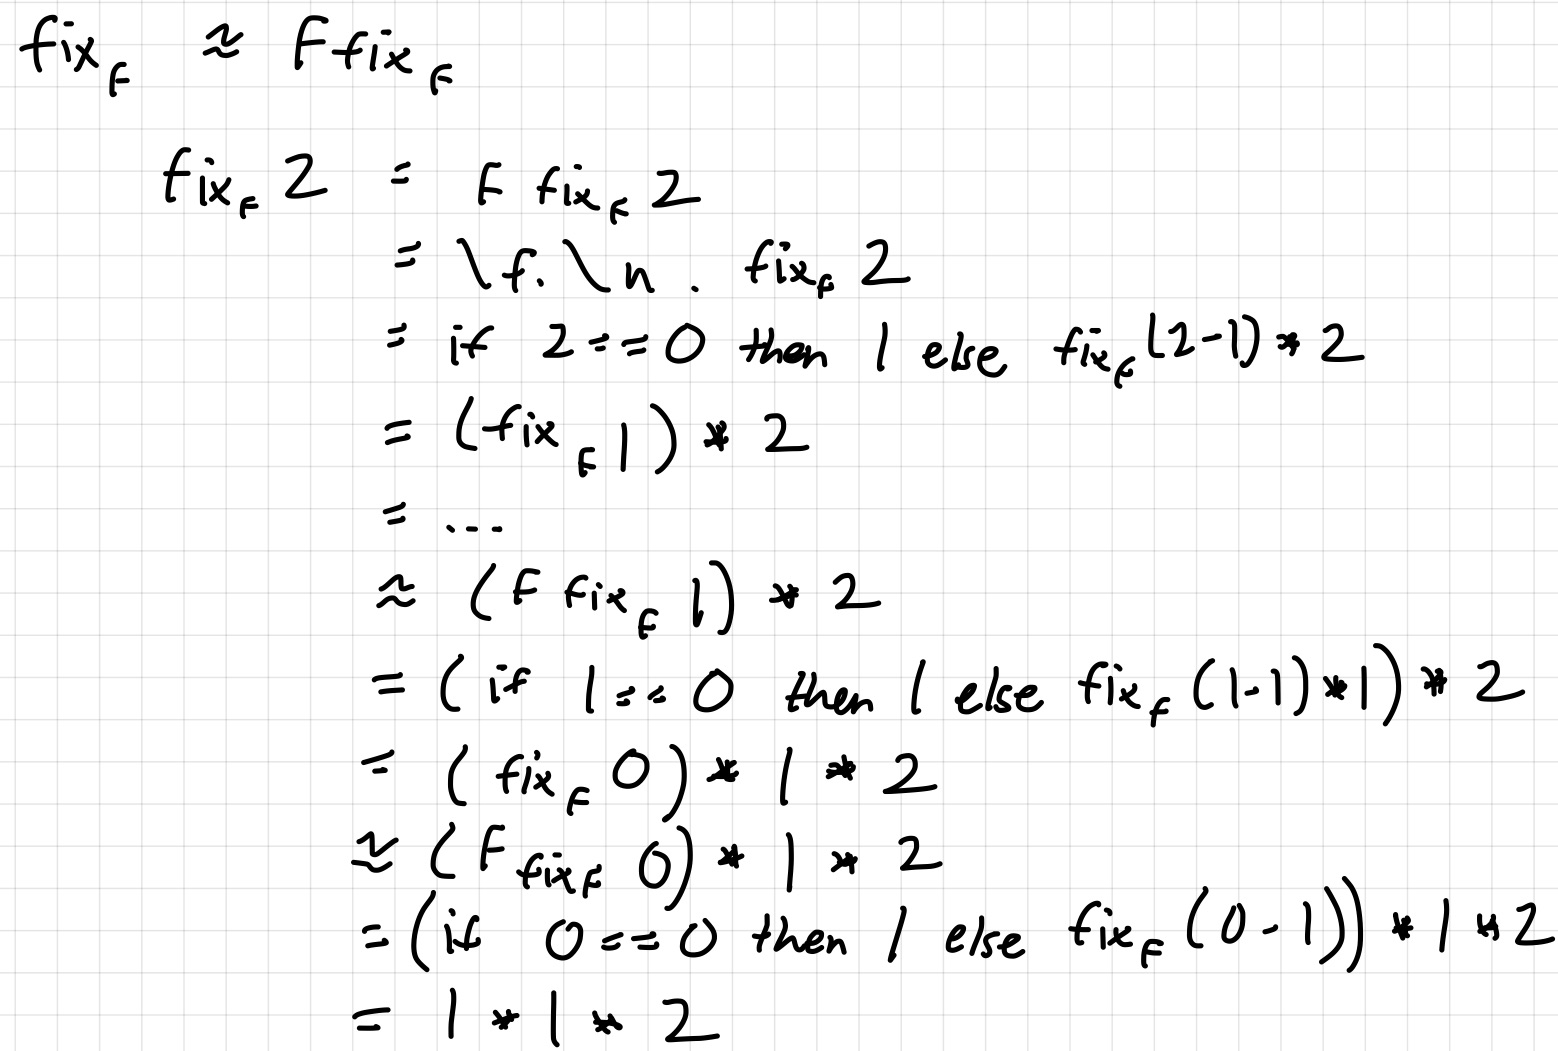
\includegraphics[width=14cm]{HW10.png}
\end{figure}

\subsection{Week 11}
For this week we analyze the article of \href{https://hackmd.io/@alexhkurz/rJ9O5tZSo}{composing contracts} as mentioned by Alex Kurz in this assignment. I then asked the following question in a discussion and replied to a few of my peers questions.

\subsubsection{My Question}
For my question, I want to focus on the section about combining contracts. What is interesting to me is that contracts can be combined, but there was no example of any type of tree that can be created through combining contracts. For example, if a contract would return some value A and from A we create another contract to return B, then another to return C this would look like A -> B -> C. This is of course assuming that all of the conditions from the contracts are being met and through combining contracts this is also combining the conditions.

Is there a transitive property that can be written to go A ->C? And if so what would the abstract syntax tree look like? This also asks another questions if there are other unexplored properties of contracts.

\subsubsection{Responses}
These are the responses to my peers.

\medskip
By Luke Boctor: Why did the creators decide to design and implement their contract valuation engine in Haskell? Could there be a better host language for their objectives?

\medskip
Answer: I believe that Haskell is chosen for this implementation because of the unique way that rules/substitution work in Haskell. In this case, contracts benefit from being able to write the equivalence relationships easily using Haskell's "=".  A contract with a condition can be resolved by simply evaluating which in Haskell is through the nature of the language to simplify the expression as much as possible using various rules. 

\medskip
By Devon Foy: Contracts aren't the only area of finance that could potentially benefit from the concepts in the paper. How could this technology be expanded on to compose and value combinations of other financial instruments such as mortgage backed securities?

\medskip
Another potential area of use could be the retail sector. It seems contracts are another way to create "trades" are ensure that a condition is fulfilled with a result at the end. For example, in a used item market where items are being sold, bought, and traded. The values of these items may not all be tracked properly and therefore contracts could be a solution to ensure all of the requirements and outputs get resolved.

\subsection{Week 12}
This week is focused on Hoarse Logic and finding invariants as well as resolving the pre/postconditions. 

\subsubsection{Condition Analysis}
The condition we will be analyzing is:
\begin{lstlisting}
while (x!=0) do z:=z*y;  x:= x-1 done
\end{lstlisting}

\medskip
To start off our analysis, we will be finding the precondition as well as the postcodition in order to get a better understanding of the problem. By looking at the equation, we can understand that x is greater than or equal to 0 because of "while (x!=0)" and we also understand that z must start at 1 so that "z=z*y" is not nullified by a 0, and therefore starts at 1 so that z is able to increase. From this, we find that the precondition would be: $$x \geq 0 \wedge z = 1$$ To find the post condition, we take a better understanding of the equation as x is the exponent of y with z being the result. In an equation this would look like: $$z = y^x$$

\subsubsection{Hoare Logic}
To find the Hoare Rule for the above while loop, we can rewrite the equation as:
$$\frac{\{I\}S\{I\}}{\{I\}while B do S done \{ \neg B \wedge I \}}$$

In this case, S represents: $$z := z * y; x:= x - 1$$ This means that I represents the while loop invariant. By doing an example of a given number, we can resolve a new invariant through using numbers. For example, if x is 10, y is 2, and z is 1, then we find that the result of this example using algebra will be $$z = 2^{(10-x)}$$ Using the precondition and postcondition as stated in the earlier section, we create $$z = y^{(t - x)}$$ where t represents the number of times the loop occurs. Replacing y with k, the invariant results to $$z = k^{(t - x)}$$

\section{Project}

For my project I will be looking into various types of programming languages and determining specific use cases and similarities between them. This project is focused on putting characteristics and attributes to programming languages and will be focused on 5-10 different languages. Some specific resources and documentation are GitHub databases.
\subsection{Specification}
The attributes to look at would be their industry/primary use, popularity, similar languages (as in what other languages do users of one language use), number of repositories, and growth/decline over the years. By doing a sentiment analysis on the Reddit page for the programming languages, (r/Python, r/C++, r/Java and so on), we use this determine which use cases are the most popular or perhaps other interesting facts about the language (such as common errors, programs, or discussion topics). This will look to create a model in which languages are popular and how they are being used.

\subsection{Prototype}
\subsection{Documentation}
\subsection{Critical Appraisal}

\ldots

\section{Conclusions}\label{conclusions}

(approx 400 words)

In the conclusion, I want a critical reflection on the content of the course. Step back from the technical details. How does the course fit into the wider world of programming languages and software engineering?

\begin{thebibliography}{99}
\bibitem[PL]{PL} \href{https://github.com/alexhkurz/programming-languages-2022/blob/main/README.md}{Programming Languages 2022}, Chapman University, 2022.
\end{thebibliography}

\end{document}
